\section{Introduction}
The Exascale Computing Project Software Technology (ECP ST) focus area represents the key bridge between Exascale systems and the scientists developing applications that will run on those platforms. ECP offers a unique opportunity to build a coherent set of software (often referred to as the ``software stack'') that will allow application developers to maximize their ability to write highly parallel applications, targeting multiple Exascale architectures with runtime environments that will provide high performance and resilience. But applications are only useful if they can provide scientific insight, and the unprecedented data produced by these applications require a complete analysis workflow that includes new technology to scalably collect, reduce, organize, curate, and analyze the data into actionable decisions. This requires approaching scientific computing in a holistic manner, encompassing the entire user workflow—from conception of a problem, setting up the problem with validated inputs, performing high-fidelity simulations, to the application of uncertainty quantification to the final analysis. The software stack plan defined here aims to address all of these needs by extending current technologies to Exascale where possible, by performing the research required to conceive of new approaches necessary to address unique problems where current approaches will not suffice, and by deploying high-quality and robust software products on the platforms developed in the Exascale systems project.
The ECP ST portfolio has established a set of interdependent projects that will allow for the research, development, and delivery of a comprehensive software stack, as summarized in Table~\ref{table:wbs}.

\begin{table}
	\begin{tabular}{|>{\columncolor[gray]{0.8}}p{0.10\linewidth}|>{\columncolor[rgb]{0.88,1,1}}p{0.15\linewidth}|p{0.6\linewidth}|}\hline
	    \vfill WBS 2.3.1\vfill & \vfill \centering{Programming Models and Runtimes} \vfill & \vfill Cross-platform, production-ready programming infrastructure to support development and scaling of mission-critical software at both the node and full-system levels.\vfill \\\hline
		\vfill WBS 2.3.2 \vfill & \vfill \centering{Development Tools} \vfill & \vfill A suite of tools and supporting unified infrastructure aimed at improving developer productivity across the software stack. This scope includes debuggers, profilers, and the supporting compiler infrastructure, with a particular emphasis on LLVM~\cite{LLVM:2018} as a delivery and deployment vehicle. \vfill \\\hline
		\vfill WBS 2.3.3 \vfill & \vfill \centering{Mathematical Libraries} \vfill & \vfill Mathematical libraries and frameworks that (i) interoperate with the ECP software stack; (ii) are incorporated into ECP applications; and (iii) provide scalable, resilient numerical algorithms that facilitate efficient simulations on Exascale computers.\vfill \\\hline
		\vfill WBS 2.3.4 \vfill & \vfill \centering{Data and Visualization} \vfill & \vfill Production infrastructure necessary to manage, share, and facilitate analysis and visualization of data in support of mission-critical codes. Data analytics and visualization software that supports scientific discovery and understanding, despite changes in hardware architecture and the size, scale, and complexity of simulation and performance data produced by Exascale platforms. \vfill \\\hline
		\vfill WBS 2.3.5 \vfill & \vfill \centering{Software Ecosystem and Delivery} \vfill & \vfill Development and coordination of Software Development Kits (SDKs), the Extreme-scale Scientific Software Stack (E4S) across all of ECP ST projects.  Development of capabilities in Spack~\cite{gamblin+:sc15} in collaboration with NNSA's primary sponsorship.  Development of SuperContainers~\cite{Supercontainers} and coordination of container-based workflows across DOE computing facilities.\vfill \\\hline
		\vfill WBS 2.3.6 \vfill & \vfill \centering{NNSA ST} \vfill & \vfill Development and enhancement of open source software capabilities that are primarily developed at Lawrence Livermore, Los Alamos and Sandia National Laboratories.  Funds for engaging open science application and software teams in the use and enhancement of these products.\vfill \\\hline
	\end{tabular}
	\caption{\label{table:wbs} ECP ST Work Breakdown Structure (WBS), Technical Area, and description of scope.}
\end{table}

ECP ST is developing a software stack to meet the needs of a broad set of Exascale applications. The current software portfolio covers many projects spanning the areas of programming models and runtimes, development tools, mathematical libraries and frameworks, data management, analysis and visualization, and software delivery. The ECP software stack was developed bottom up based on application requirements and the existing software stack at DOE HPC Facilities. The portfolio comprises projects selected in two different ways: 
\begin{enumerate}
\item Thirty projects funded by the DOE Office of Science (ASCR).  This scope of work was selected in October 2016 via an RFI and RFP process, considering prioritized requirements. The initial collection of loosely coupled projects has been re-organized twice and is now in a form that should serve us well as we move to the more formal execution phases of the project.
\item Three DOE NNSA/ASC funded projects that are part of the Advanced Technology Development and Mitigation (ATDM) program, which is in its sixth year (started in FY14). These projects are focused on longer term research to address the shift in computing technology to extreme, heterogeneous architectures and to advance the capabilities of NNSA/ASC simulation codes. 
\end{enumerate}
Since the initial selection process, ECP ST has reorganized efforts as described in Section~\ref{subsect:ProjectRestructuring}.

\begin{figure}
	\centering
	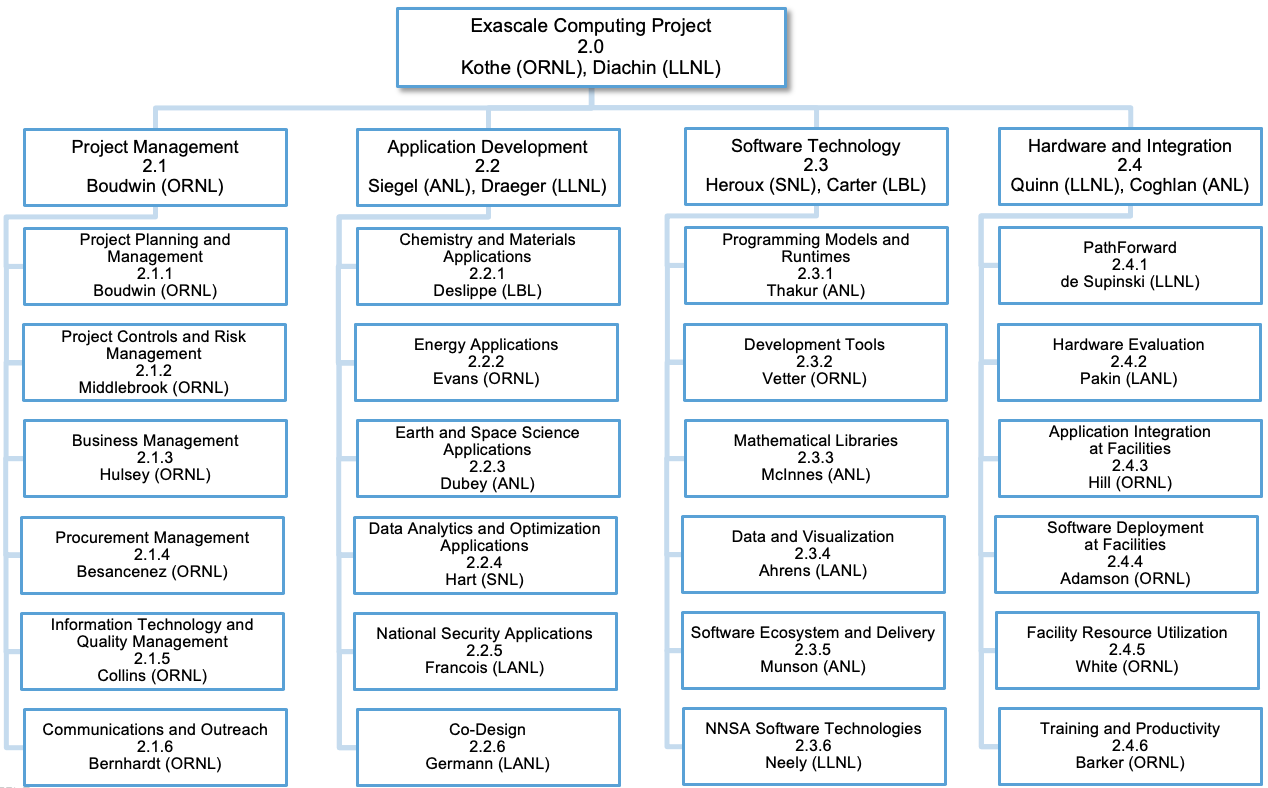
\includegraphics[width=0.9\linewidth]{ECP21}
	\caption{The ECP Work Breakdown Structure through Level 3 (L3) as of December 5, 2019. Under Software Technology, WBS 2.3.6 consolidates ATDM contributions to ECP into a new L3 area.}
	\label{fig:ecp2}
\end{figure}

\subsection{Background}
Historically, the software used on supercomputers has come from three sources: computer system vendors, DOE laboratories, and academia. Traditionally, vendors have supplied system software:  operating system, compilers, runtime, and system-management software. The basic system software is typically augmented by software developed by the DOE HPC facilities to fill gaps or to improve management of the systems. An observation is that it is common for system software to break or not perform well when there is a jump in the scale of the system.
 
Mathematical libraries and tools for supercomputers have traditionally been developed at DOE laboratories and universities and ported to the new computer architectures when they are deployed. These math libraries and tools have been remarkably robust and have supplied some of the most impactful improvements in application performance and productivity. The challenges have been the constant adapting and tuning to rapidly changing architectures.
 
Programming paradigms and the associated programming environments that include compilers, debuggers, message passing, and associated runtimes have traditionally been developed by vendors, DOE laboratories, and universities. The same can be said for file system and storage software. An observation is that the vendor is ultimately responsible for providing a programming environment and file system with the supercomputer, but there is often a struggle to get the vendors to support software developed by others or to invest in new ideas that have few or no users yet. Another observation is that file-system software plays a key role in overall system resilience, and the difficulty of making the file-system software resilient has grown non-linearly with the scale and complexity of the supercomputers.
 
In addition to the lessons learned from traditional approaches, Exascale computers pose unique software challenges including the following.
\begin{itemize}
\item \textbf{Extreme parallelism:} Experience has shown that software breaks at each shift in scale. Exascale systems are predicted to have a billion-way concurrency almost exclusively from discrete accelerator devices, similar to today's GPUs. Because clock speeds have essentially stalled, the 1000-fold increase in potential performance going from Petascale to Exascale is entirely from concurrency improvements.
\item \textbf{Data movement in a deep memory hierarchy: }Data movement has been identified as a key impediment to performance and power consumption. Exascale system designs are increasing the types and layers of memory, which further challenges the software to increase data locality and reuse, while reducing data movement.
\item \textbf{Discrete memory and execution spaces:} The node architectures of Exascale systems include host CPUs and discrete device accelerators.  Programming for these systems requires coordinated transfer of data and work between the host and device. While some of this transfer can be managed implicitly, for the most performance-sensitive phases, the programmer typically must manage host-device coordination explicitly.  Much of the software transformation effort will be focused on this issue.
\end{itemize}
 
In addition to the software challenges imposed by the scale of Exascale computers, the following additional requirements push ECP away from the historical approaches for getting the needed software for DOE supercomputers.
\begin{itemize}
\item \textbf{2021 acceleration:} ECP has a goal of accelerating the development of the U.S. Exascale systems and enabling the first deployment by 2021. This means that the software needs to be ready sooner, and the approach of just waiting until it is ready will not work. A concerted plan that accelerates the development of the highest priority and most impactful software is needed.
\item \textbf{Productivity:} Traditional supercomputer software requires a great deal of expertise to use. ECP has a goal of making Exascale computing accessible to a wider science community than previous supercomputers have been. This requires the development of software that improves productivity and ease of use.
\item \textbf{Diversity:} There is a strong push to make software run across diverse Exascale systems. Accelerator devices from Nvidia have been available for many years and specific host-device programming and execution applications have been successfully ported to these platforms.  Exascale platforms will continue to have this kind of execution model, but with different programming and runtime software stacks.  Writing high-performance, portable code for these platforms will be challenging.
\item \textbf{Analytics and machine learning:} Future DOE supercomputers will need to solve emerging data science and machine learning problems in addition to the traditional modeling and simulation applications. This will require the development of scalable, parallel analytics and machine learning software for scientific applications, much of which does not exist today.
\end{itemize}
 
The next section describes the approach employed by ECP ST to address the Exascale challenges.

\subsection{ECP ST Project Restructuring}\label{subsect:ProjectRestructuring}

The initial organization of ECP ST was based on discussions that occurred over several years of Exascale planning within DOE, especially the DOE Office of Advanced Scientific Computing Research (ASCR).  Figure~\ref{fig:ecpstv1} shows the conceptual diagram of this first phase.  The 66 ECP ST projects were mapped into 8 technical areas, in some cases arbitrating where a project should go based on its primary type of work, even if other work was present in the project.  In November 2017, ECP ST was reorganized into 5 technical areas, primarily through merging a few smaller areas, and the number of projects was reduced to 56 (then 55 due to further merging in \ecosystem).  Figure~\ref{fig:ecpstv2} shows the diagram of the second phase of ECP ST.  In Section~\ref{sect:PETA}, we describe the organization, planning, execution, tracking and assessment processes that will put ECP ST in a good position for success in the CD-2 phase of the project.

\begin{figure}
	\centering
	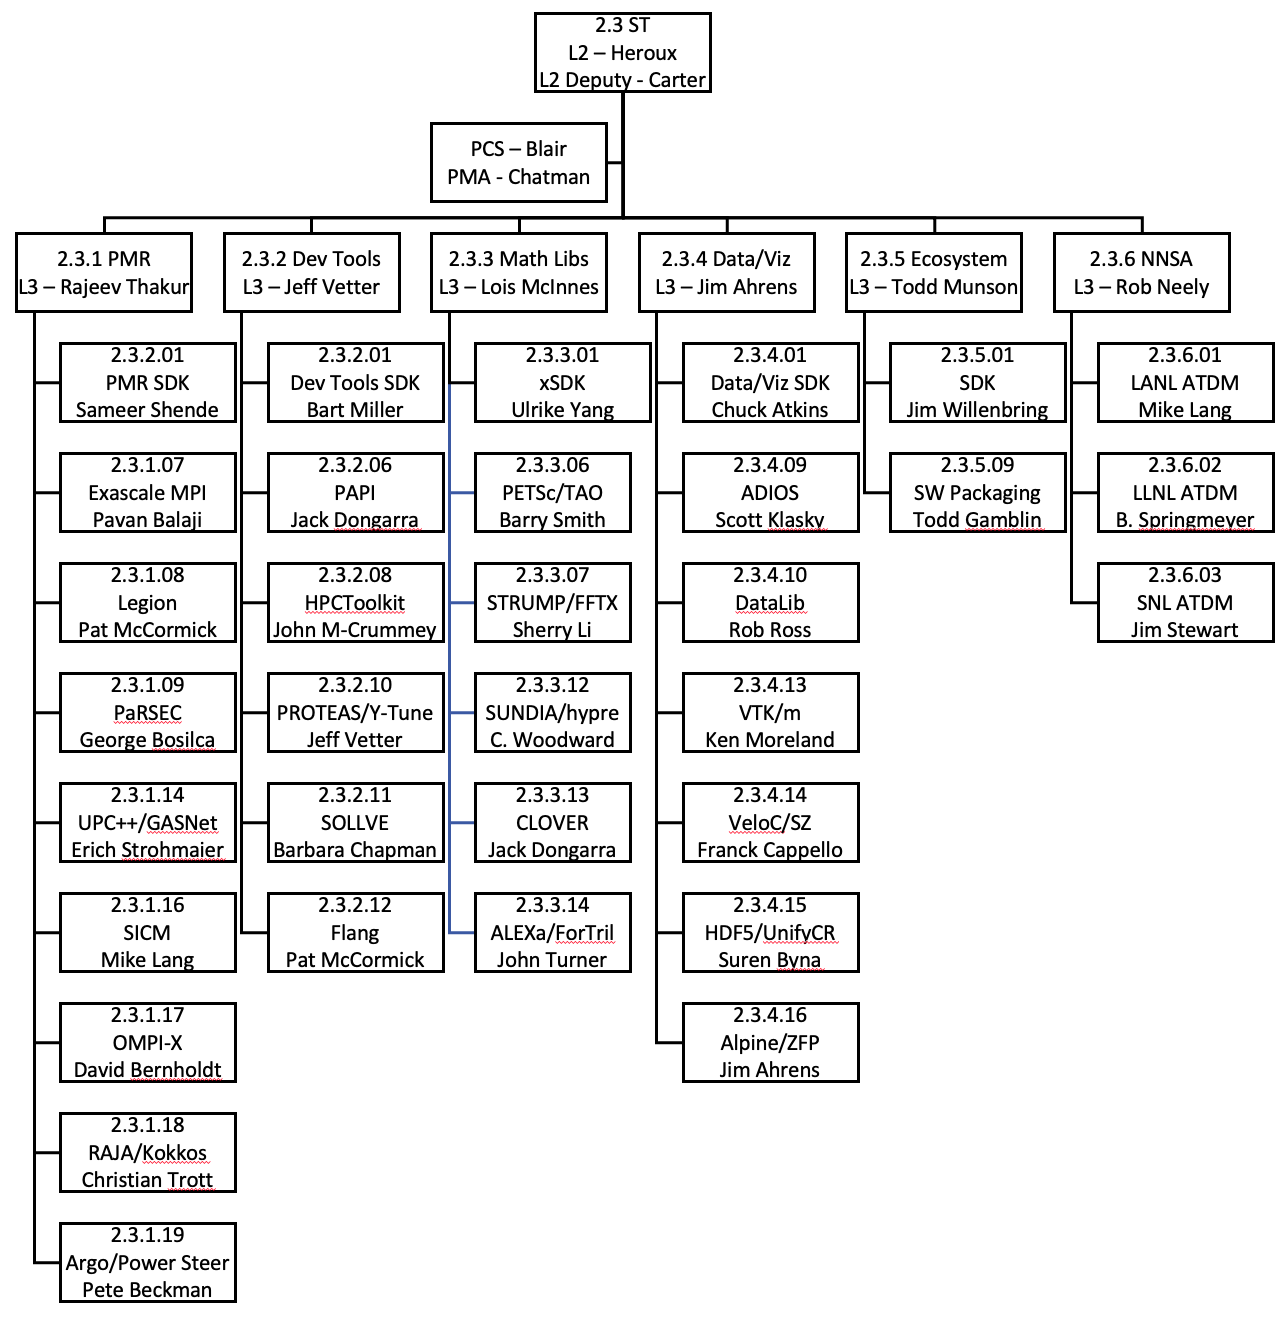
\includegraphics[width=0.9\linewidth]{STFY20WBS}
	\caption{\label{fig:wbs-FY20} The FY20 ECP ST WBS structure as of December 5, 2019, includes a new L3 (2.3.6) and better balances L4 subprojects in the first four L3 technical areas.  Technical area 2.3.5 has only two projects, which are focused on meta-product development in SDKs, E4S, Spack and SuperContainers.}
\end{figure}

\begin{figure}
\begin{mdframed}
\begin{itemize}
\item Phase 1: 66 total L4 subprojects
\begin{itemize}
\item 35 projects funded by the DOE Office of Science that were selected in late 2016 via an RFI and RFP process, considering prioritized requirements of applications and DOE facilities. 
These projects started work in January–March 2017 depending on when the contracts were awarded.
\item 31 ongoing DOE NNSA funded projects that are part of the Advanced Technology Development and Mitigation (ATDM) program. The ATDM program started in FY14.  These projects are focused on longer term research to address the shift in computing technology to extreme, heterogeneous architectures and to advance the capabilities of NNSA simulation codes.
\end{itemize}
\item Phase 2: 55 total L4 subprojects
\begin{itemize}
\item 41 ASCR-funded projects.  Added  2 \ecosystem\ projects and 4 SDK projects.
\item 15 ATDM projects: Combined the previous 31 ATDM projects into one project per technical area per lab.  ATDM projects are generally more vertically integrated and would not perfectly map to any proposed ECP ST technical structure.  Minimizing the number of ATDM projects within the ECP WBS structure reduces complexity of ATDM to ECP coordination and gives ATDM flexibility in revising its portfolio without disruption to the ECP-ATDM mapping.
\end{itemize}
\item Phase 3: 33 total L4 subprojects.  Fewer, larger and more uniform-sized projects
\begin{itemize}
	\item Starting with FY2020, ECP ST has further consolidated L4 projects to foster additional synergies and amortize project overheads as ECP heads into Critical Decision Phase 2~\cite{413.3B}, where more rigor in planning and execution are needed.
	\item 5 L3s to 6: New NNSA ST L3
	\item 40 ST SC-funded L4 subprojects to 30.
	\begin{itemize}
	\item \pmr – 13 to 9, \tools - 6 to 6, \mathlibs - 7 to 6, \dataviz - 10 to 7, \ecosystem - 4 to 3.
	\item Includes 2 new L4 subprojects in SW Ecosystem.
	\end{itemize}
	\item 15 ST NNSA-funded projects transferred to new NNSA ST L3. Consolidated from 15 to 3 L4 subprojects.
	\item No more small subprojects.
	\item Figure~\ref{fig:wbs-FY20} show the overall structure.
\end{itemize}
\end{itemize}
\end{mdframed}

\caption{\label{fig:project-remapping}Project remapping summary from Phase 1 (through November 2017) to Phase 2 (November 2017 -- September 30, 2019) to Phase 3 (After October 1, 2019)}
\end{figure}


\begin{figure}
	\centering
	\includegraphics[width=0.9\linewidth]{ECPSTV1}
	\caption{ECP ST before November 2017 reorganization.  This conceptually layout emerged from several years of Exascale planning, conducted primarily within the DOE Office of Advanced Scientific Computing Research (ASCR).  After a significant restructuring of ECP that removed much of the facilities activities and reduced the project timeline from 10 to seven years, and a growing awareness of what risks had diminished, this diagram no longer represented ECP ST efforts accurately.}
	\label{fig:ecpstv1}
\end{figure}
\begin{figure}
	\centering
	\includegraphics[width=0.9\linewidth]{ECPSTV2}
	\caption{ECP ST after November 2017 reorganization.  This diagram more accurately reflects the priorities and efforts of ECP ST given the new ECP project scope and the demands that we foresee.}
	\label{fig:ecpstv2}
\end{figure}
\begin{figure}
	\centering
	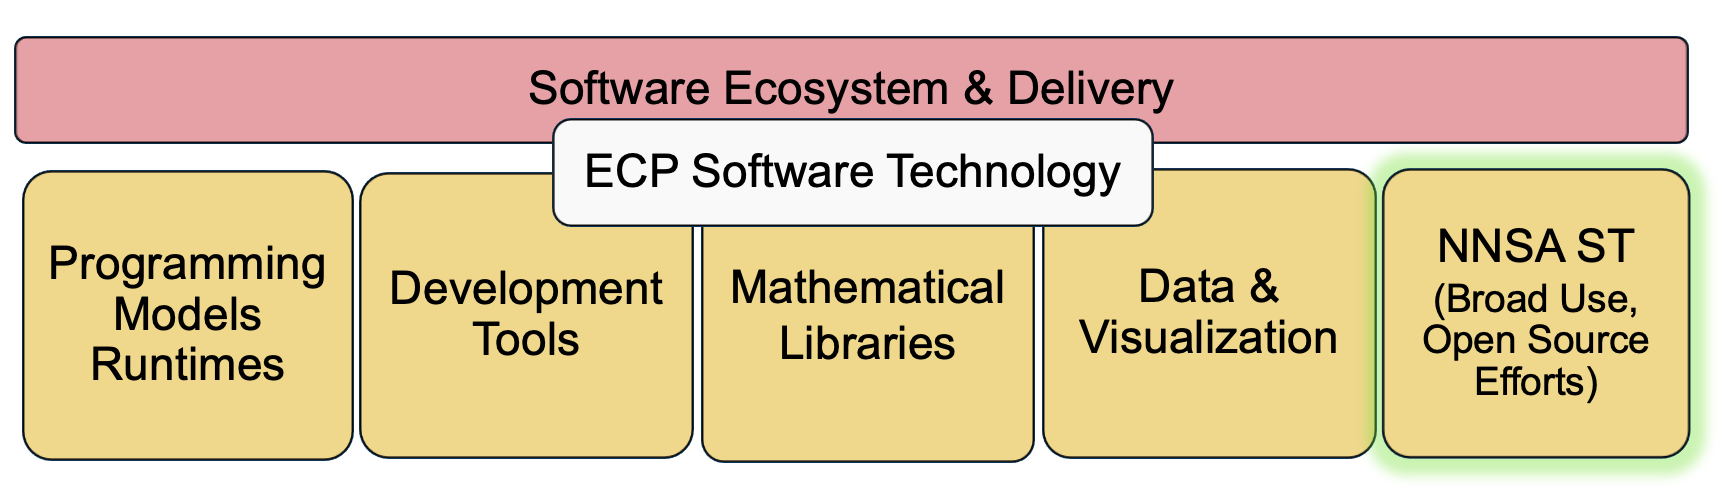
\includegraphics[width=0.9\linewidth]{ECPSTV3}
	\caption{ECP ST after October 2019 reorganization.  This diagram reflects the further consolidation of NNSA open source contributions to enable more flexible management of NNSA ST contributions.}
\end{figure}
\begin{figure}
	\centering
	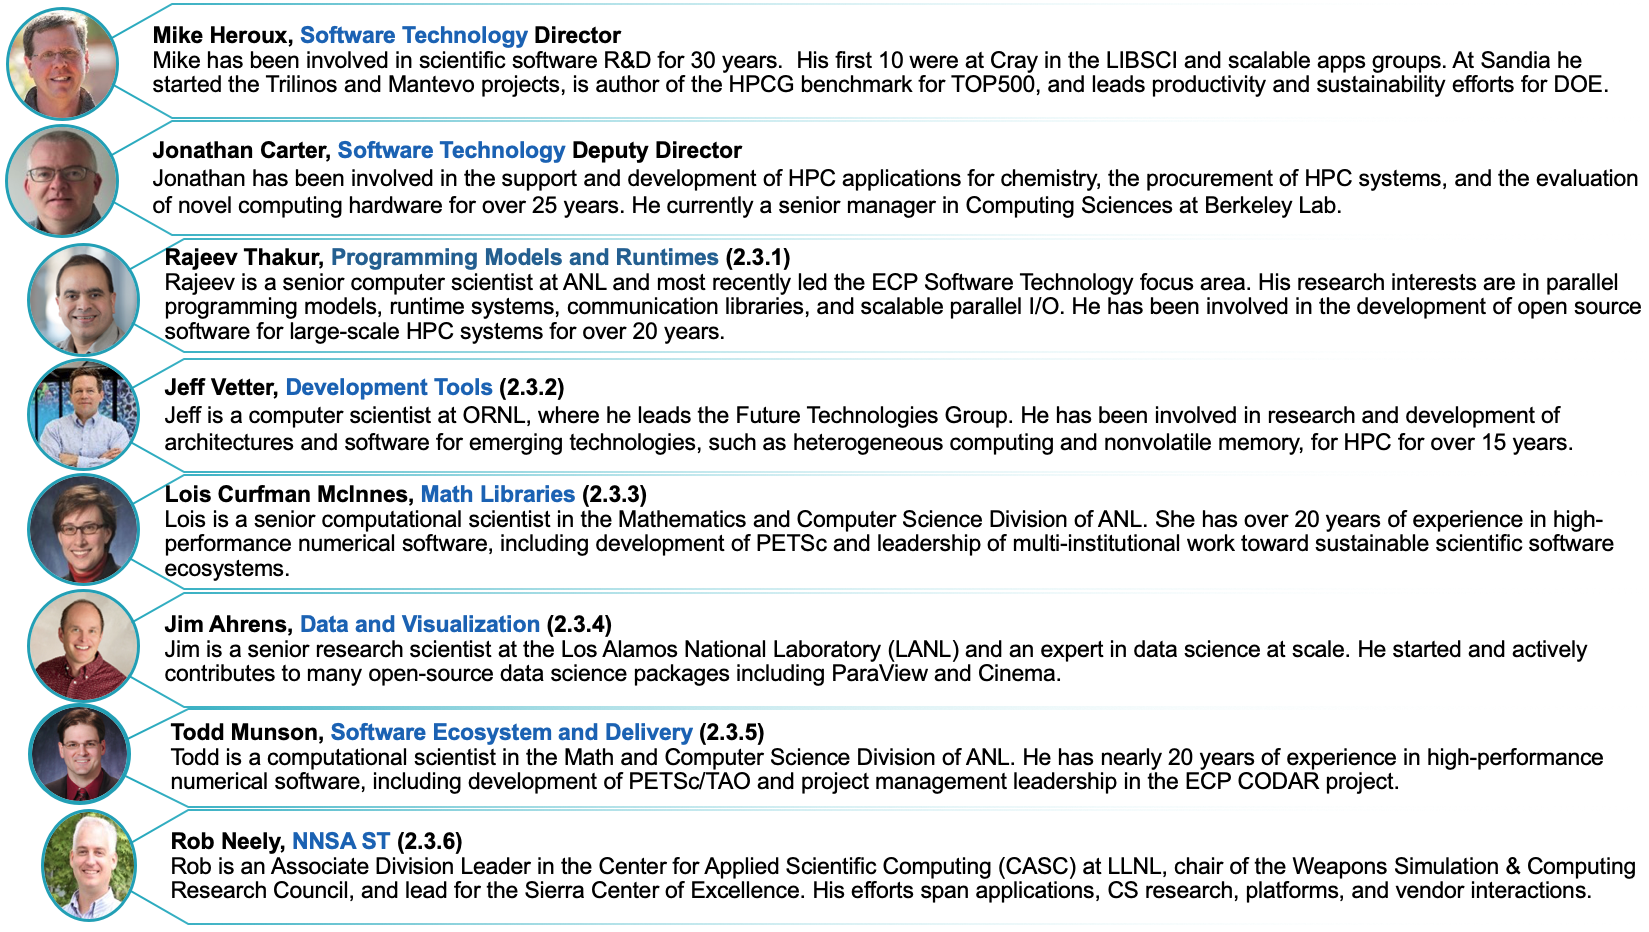
\includegraphics[width=0.9\linewidth]{ECP-ST-Leads}
	\caption{ECP ST Leadership Team as of October 2019.}
	\label{fig:ecpstleads}
\end{figure}

